%%%%%%%%%%%%%%%%%%%%%%%%%%%%%%%%%%%%
% Appendix A, Solution and Estimation Details
%%%%%%%%%%%%%%%%%%%%%%%%%%%%%%%%%%%%

% Set equation, figure, table indexing
\renewcommand{\thefigure}{A.\arabic{figure}}
\setcounter{figure}{0}
\renewcommand{\thetable}{A.\arabic{table}}
\setcounter{table}{0}
\renewcommand{\theequation}{A.\arabic{equation}}
\setcounter{equation}{0}
\renewcommand{\thefootnote}{A.\arabic{footnote}}
\setcounter{footnote}{0}

\section{Tables}\label{appendix:tabs}

\begin{landscape}
\begin{table}[H]
\centering
\begin{threeparttable}
\caption{Multiple-Testing Adjustment for the Primary Family of Per-Capita Effects}
\label{atab:qvalues}
\begin{tabular}{lcccc}
\toprule
 & \multicolumn{2}{c}{Clustered} & \multicolumn{2}{c}{Randomization inference} \\
\cmidrule(lr){2-3} \cmidrule(lr){4-5}
Hypothesis (avg.\ post effect, matched per 100{,}000) & $p$-value & $q$-value & $p$-value & $q$-value \\
\midrule
Full sample (headline) & 0.103 & 0.123 & 0.579 & 0.762 \\
Urban hospitals & 0.095 & 0.123 & 0.635 & 0.762 \\
Rural hospitals & $<$0.001 & 0.002 & 0.289 & 0.762 \\
Primary care & 0.063 & 0.123 & 0.762 & 0.762 \\
Non-primary care & 0.219 & 0.219 & 0.475 & 0.762 \\
Offered positions (quota) & 0.033 & 0.098 & 0.515 & 0.762 \\
\bottomrule
\end{tabular}

\begin{tablenotes}\footnotesize
\item \textit{Notes:} The table reports Benjamini--Hochberg false-discovery-rate $q$-values for the primary family of average post-expansion effects on matched positions per 100{,}000 population, computed under two inference standards. ``Clustered'' $p$-values are the joint tests of the post-expansion event-time coefficients with standard errors clustered at the state level (the offered-positions row uses the quota outcome). ``Randomization inference'' $p$-values permute the vector of state expansion-timing cohorts across the states in each specification's sample under the sharp null of no effect ($1{,}000$ permutation draws for the full-sample headline, $500$ for the other members) and compare the observed average post effect with the permutation distribution; this is the conservative standard the text leads with, applied uniformly to every family member. Within each standard, $q$-values apply the Benjamini--Hochberg correction across the family of six tests; a $q$-value below $0.05$ indicates a finding that survives a $5$ percent false-discovery-rate correction.
\end{tablenotes}
\end{threeparttable}
\end{table}

\begin{table}[H]
\centering
\singlespacing
\small
\begin{threeparttable}
\caption{Baseline Balance Across Medicaid GME Formula Groups (2010)}
\label{atab:balance}
\begin{tabular}{>{\raggedright\arraybackslash}p{3in}ccccc}
\toprule
 & Volume- & Fixed/ & Never- & Difference & \\
Baseline characteristic (2010) & responsive & none & expansion & (1)$-$(2) & $p$-value \\
 & (1) & (2) & (3) & & \\
\midrule
Matched positions per program & 33.6 & 33.8 & 37.0 & -0.3 & 0.960 \\
Offered positions (quota) per program & 35.8 & 35.6 & 38.8 & 0.2 & 0.963 \\
Share of programs filling every offered position & 0.81 & 0.79 & 0.87 & 0.02 & 0.767 \\
Matched positions per 100{,}000 population & 10.25 & 8.26 & 5.46 & 1.99 & 0.594 \\
\quad Program-level mean, population-weighted & 0.49 & 0.23 & 0.37 & 0.26 & -- \\
Offered positions (quota) per 100{,}000 & 10.80 & 8.64 & 5.76 & 2.16 & 0.571 \\
Number of programs & 10.3 & 19.0 & 8.9 & -8.7 & 0.140 \\
State population (millions) & 4.2 & 7.4 & 6.3 & -3.2 & 0.177 \\
Rural program share & 0.06 & 0.07 & 0.08 & -0.01 & 0.819 \\
Primary-care share of matched positions & 0.52 & 0.55 & 0.57 & -0.03 & 0.478 \\
Mean expansion year & 2014.5 & 2014.5 & -- & 0.0 & 1.000 \\
\midrule
Number of states & 16 & 18 & 17 & & \\
\bottomrule
\end{tabular}

\begin{tablenotes}\footnotesize
\item \textit{Notes:} The table reports baseline (2010, pre-treatment) means by Medicaid GME formula group, for the same characteristics as the summary-statistics table (\cref{tab:sumstats}). Expansion states are classified as volume-responsive or fixed/none from the payment methodology reported in the 2012 survey of \textcite{henderson2013}; never-expansion states are shown for reference. All rows except the population-weighted row are unweighted means across states (the state is the unit of observation); the $p$-value is from a Welch two-sample $t$-test of the volume-responsive versus fixed/none difference at the state level, so power is limited by the number of states. The population-weighted row reports the program-level mean of matched positions per 100{,}000 (2010 population), weighted by state population---the object the estimation weights by; its cross-group gap reflects the concentration of training in a few large volume-responsive states rather than state-level imbalance. The fill-share row is measured at the NRMP specialty-program level (the share of a state's specialty programs filling every offered position); the primary-care share is the share of matched positions in family medicine, internal medicine, and pediatrics; rural programs are those in counties with 2010 RUCA codes above 3. Data are from NRMP Main Residency Match reports and the U.S.\ Census Bureau.
\end{tablenotes}
\end{threeparttable}
\end{table}
\end{landscape}
\begin{figure}[H]
    \caption{Average Post-Expansion Effects and False-Discovery-Rate Significance Across the Primary Family}
    \label{afig:fdrforest}
    \centering
      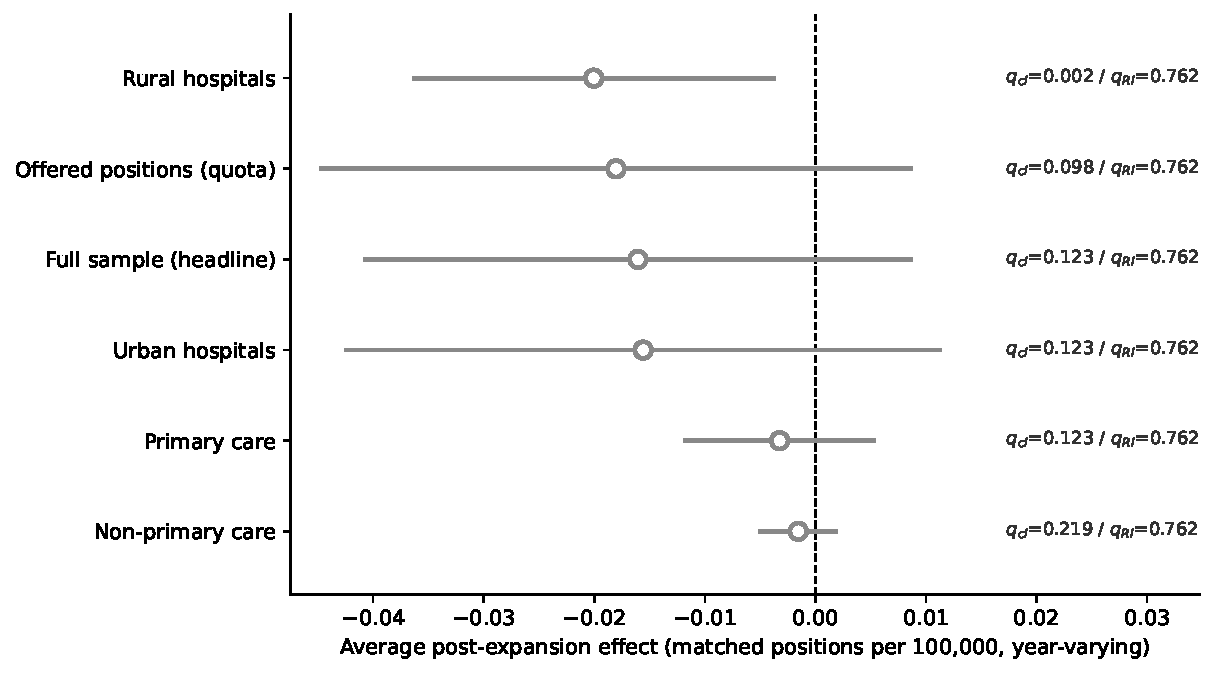
\includegraphics[width=0.85\linewidth]{figures/appx-fdr-forest.pdf}
    \hfill
\caption*{\footnotesize{\textit{Notes:} The figure plots the average post-expansion effect on matched positions per 100{,}000 contemporary (year-varying) population for each member of the primary family of hypotheses, with 95 percent confidence intervals (point estimate $\pm 1.96$ clustered standard errors). The label beside each marker reports the Benjamini--Hochberg false-discovery-rate $q$-value under both inference standards: $q_{cl}$ (clustered) and $q_{RI}$ (randomization inference). Filled markers would denote effects surviving a $5$ percent false-discovery-rate correction under the conservative randomization standard; no member survives it ($q_{RI} \geq 0.76$). Under clustered inference the rural effect is the lone survivor ($q = 0.002$), a result we discount because the rural subsample fails its own pre-trends test (see \cref{subsec:location}). Standard errors are clustered at the state level.}}
\end{figure}

\newpage
\pagebreak

\section{Figures}\label{appendix:figs}

\begin{figure}[H]
    \caption{Effect of Medicaid Expansion on Matched Residency Positions in Levels: Event Study Estimates}
    \label{afig1}
    \centering
      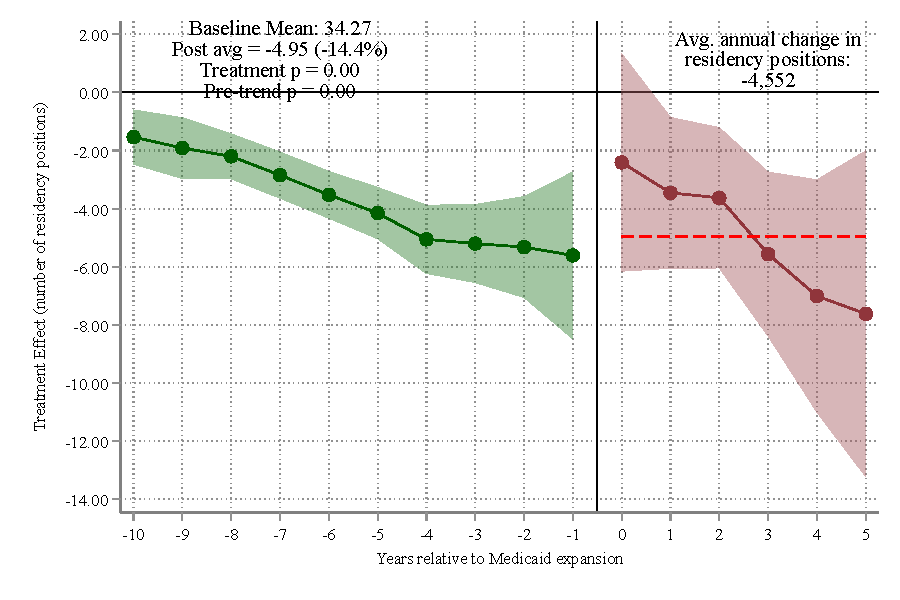
\includegraphics[width=\linewidth]{figures/appx-levels-headline.pdf}
    \hfill
\caption*{\footnotesize{\textit{Notes:} The figure plots event-study coefficients from the imputation estimator of Borusyak, Jaravel, and Spiess (2024), where the outcome is the absolute number of matched residency positions per hospital (not normalized by population). The horizontal axis measures years relative to a state's Medicaid expansion; year 0 is the first year of expansion. Green circles (years $-5$ to $-1$) show pre-expansion coefficients; dark red circles (years $0$ to $+5$) show post-expansion treatment effects. The dashed red line indicates the average post-expansion treatment effect of $-3.85$ positions per hospital, corresponding to a $13.1$ percent decline relative to the pre-expansion mean of $29.43$ matched positions (p $< 0.01$). \textbf{The pre-expansion coefficients in this raw-count specification are large and negative} (on the order of $-2$ positions per hospital, comparable in magnitude to the treatment effect), indicating a violation of parallel trends. This levels estimate therefore corroborates the \emph{direction} of the effect but should not be read as a clean causal magnitude; the paper's primary specification instead normalizes by contemporary population, which restores flat pre-trends (see \cref{subsec:inference}). Shaded bands are 95 percent confidence intervals. Regressions include hospital and year fixed effects. Standard errors are clustered at the state level.}}
\end{figure}

\begin{figure}[H]
    \caption{Effect of Medicaid Expansion on Offered Residency Positions (Quota): Event Study Estimates}
    \label{afig2}
    \centering
      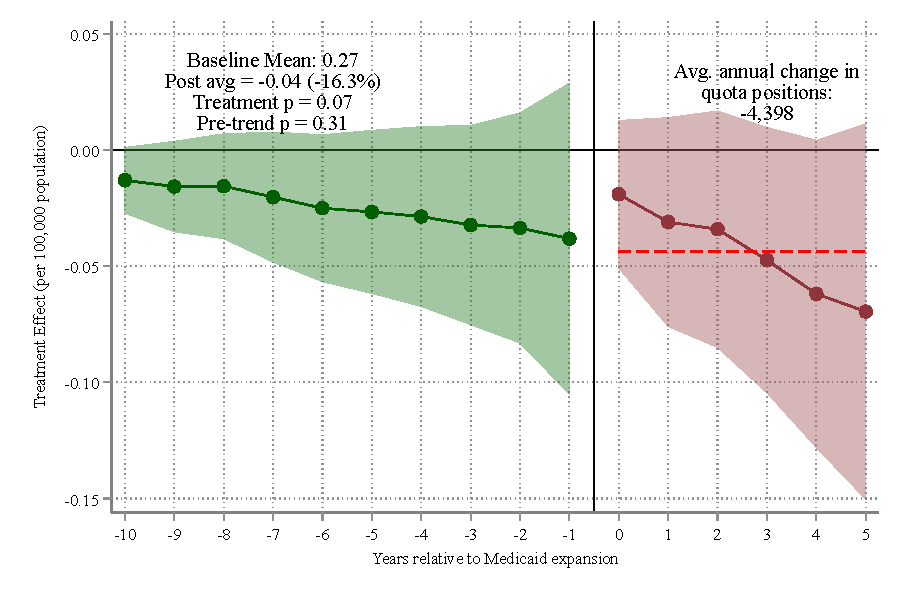
\includegraphics[width=\linewidth]{figures/appx-quota-headline.pdf}
    \hfill
\caption*{\footnotesize{\textit{Notes:} The figure plots event-study coefficients from the imputation estimator of Borusyak, Jaravel, and Spiess (2024), where the outcome is quota positions per 100,000 state population (fixed 2010 population; the year-varying quota estimate of $-0.018$ is reported in the text). Quota positions are the number of positions offered by residency programs in the NRMP Main Residency Match, prior to the matching algorithm; matched positions (the primary outcome in \cref{fig5}) are the subset of offered positions that are ultimately filled. The average post-expansion treatment effect is $-0.03$ ($-13.1$ percent relative to the pre-expansion mean of $0.23$ offered positions per 100,000; p $= 0.01$), corresponding to an average annual reduction of approximately $2{,}771$ offered positions nationally. Shaded bands are 95 percent confidence intervals. Regressions include hospital and year fixed effects. Standard errors are clustered at the state level.}}
\end{figure}

\begin{figure}[H]
    \caption{Effect of Medicaid Expansion on Matched Residency Positions by Hospital Location, in Levels: Event Study Estimates}
    \label{afig3}
    \centering
      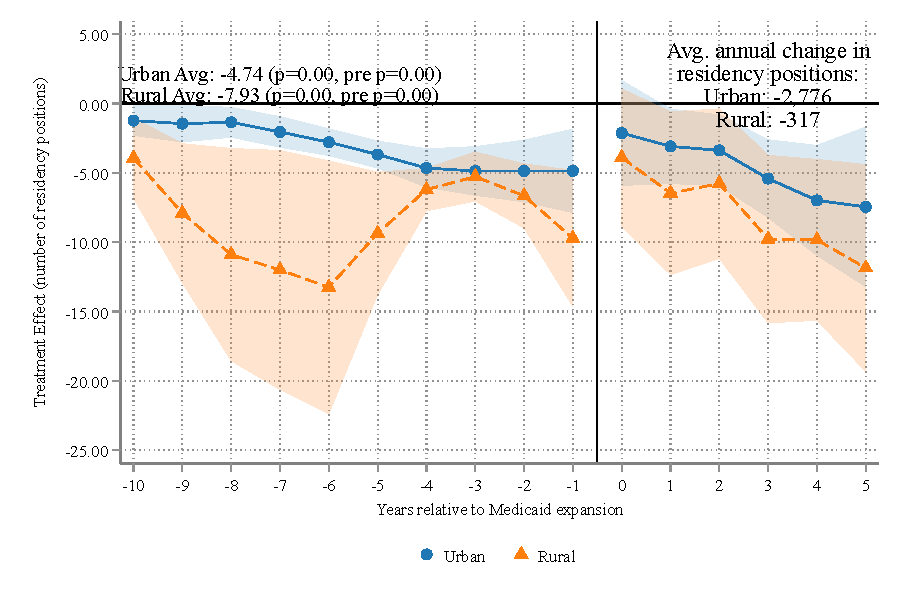
\includegraphics[width=\linewidth]{figures/appx-levels-location.pdf}
    \hfill
\caption*{\footnotesize{\textit{Notes:} The figure plots event-study coefficients from the imputation estimator of Borusyak, Jaravel, and Spiess (2024), estimated in two split-sample regressions for urban (blue circles) and rural (orange triangles) hospitals; each subsample keeps the never-expansion hospitals of its own type as the comparison group, so each series carries its own pre-expansion path and pre-trends test. The outcome is the absolute number of matched residency positions per hospital (not normalized by population). The average post-expansion treatment effect is $-3.62$ positions per hospital for urban hospitals (joint p $< 0.001$; pre-trend p $< 0.001$) and $-8.44$ positions per hospital for rural hospitals (joint p $< 0.001$; pre-trend p $= 0.02$). As with the aggregate levels outcome (\cref{afig1}), both subsamples fail the pre-trends test in levels, so these magnitudes corroborate the direction of the effect only. Translating to aggregate counts, expansion states experienced average annual reductions of approximately $2{,}120$ matched positions at urban hospitals and $338$ at rural hospitals. Shaded bands are 95 percent confidence intervals. Regressions include hospital and year fixed effects and weight by 2010 state population. Standard errors are clustered at the state level.}}
\end{figure}

\begin{figure}[H]
    \caption{Effect of Medicaid Expansion on Offered Residency Positions (Quota) by Hospital Location: Event Study Estimates}
    \label{afig4}
    \centering
      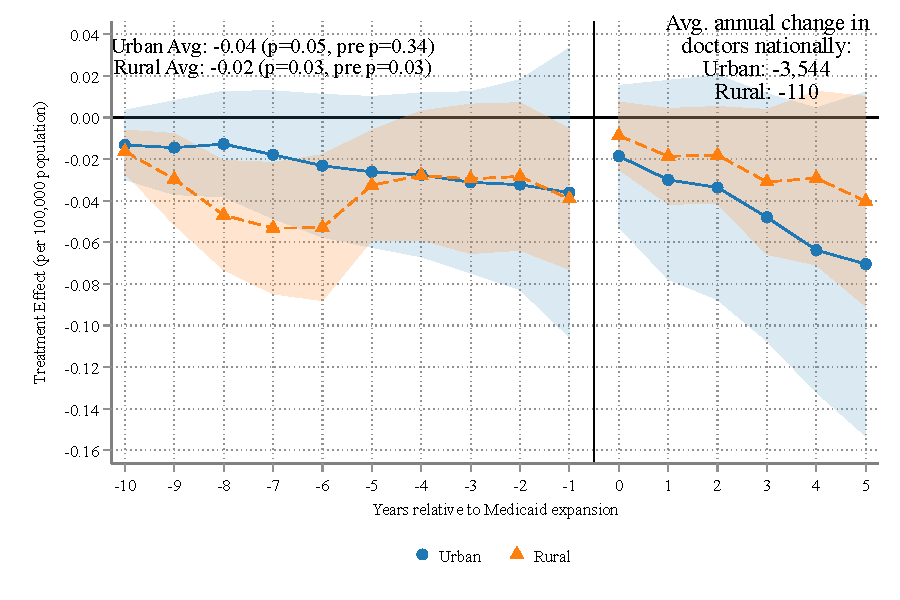
\includegraphics[width=\linewidth]{figures/appx-quota-location.pdf}
    \hfill
\caption*{\footnotesize{\textit{Notes:} The figure plots event-study coefficients from the imputation estimator of Borusyak, Jaravel, and Spiess (2024), estimated in two split-sample regressions for urban (blue circles) and rural (orange triangles) hospitals; each subsample keeps the never-expansion hospitals of its own type as the comparison group, so each series carries its own pre-expansion path and pre-trends test. The outcome is quota positions per 100,000 state population (fixed 2010 population), where quota measures positions offered by programs prior to the matching algorithm. The average post-expansion treatment effect is $-0.031$ for urban hospitals (joint p $= 0.03$; pre-trend p $= 0.10$) and $-0.026$ for rural hospitals (joint p $= 0.03$), similar in magnitude across the two groups. The rural subsample fails its own pre-trends test (p $< 0.001$), so the rural series should be read descriptively. These estimates correspond to average annual reductions of approximately $2{,}452$ offered positions at urban hospitals and $118$ at rural hospitals. Shaded bands are 95 percent confidence intervals. Regressions include hospital and year fixed effects and weight by 2010 state population. Standard errors are clustered at the state level.}}
\end{figure}

\begin{figure}[H]
    \caption{Effect of Medicaid Expansion on Matched Residency Positions by Specialty Type, in Levels: Event Study Estimates}
    \label{afig5}
    \centering
    \begin{subfigure}{\linewidth}
        \centering
        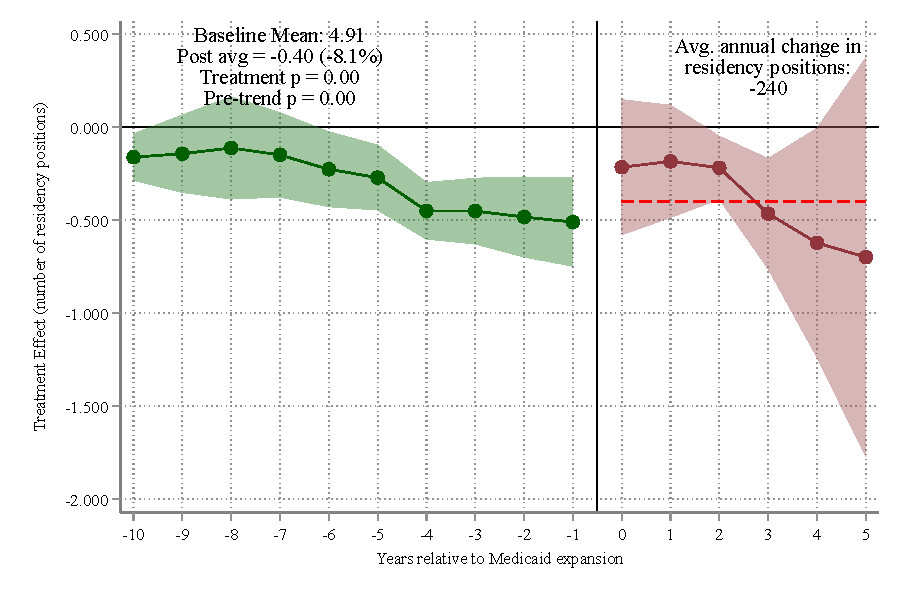
\includegraphics[width=0.75\linewidth]{figures/appx-levels-specialty-nonprimary.pdf}
        \caption{Non-Primary Care Positions}
        \label{afig5:non-prim-care}
    \end{subfigure}
    \hfill
    \begin{subfigure}{\linewidth}
        \centering
        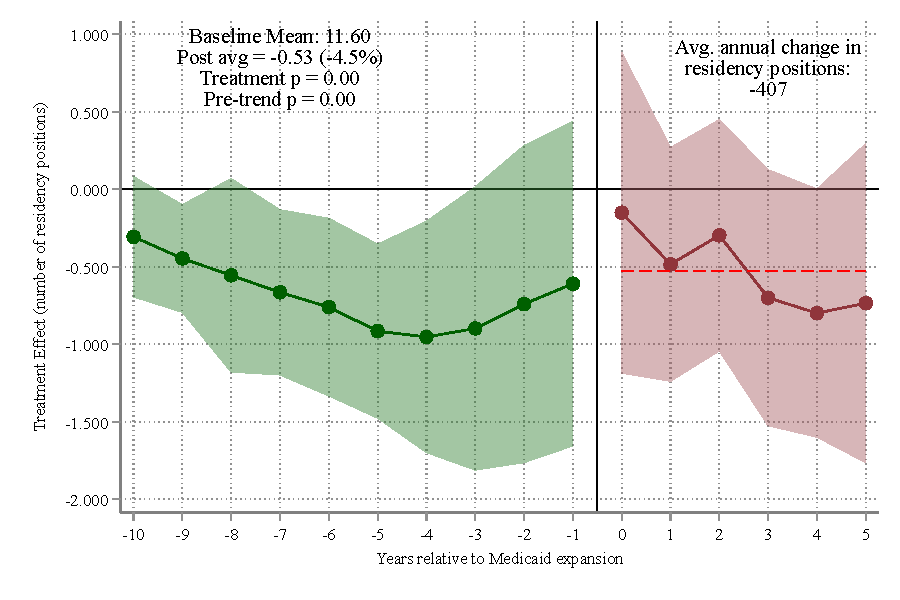
\includegraphics[width=0.75\linewidth]{figures/appx-levels-specialty-primary.pdf}
        \caption{Primary Care Positions}
        \label{afig5:prim-care}
    \end{subfigure}
\caption*{\footnotesize{\textit{Notes:} The figure plots event-study coefficients from the imputation estimator of Borusyak, Jaravel, and Spiess (2024), estimated separately for non-primary care (top panel) and primary care specialties (bottom panel). The outcome is the absolute number of matched residency positions per hospital (not normalized by population). Primary care includes family medicine, internal medicine, and pediatrics. The average post-expansion treatment effect is $-0.37$ positions per hospital for non-primary care ($-8.6$ percent relative to the pre-expansion mean of $4.37$; p $< 0.01$), corresponding to an average annual reduction of approximately $155$ matched positions nationally. For primary care, the average treatment effect is $-0.95$ positions per hospital ($-10.0$ percent relative to the pre-expansion mean of $9.52$; p $< 0.01$), corresponding to an average annual reduction of approximately $562$ positions. Shaded bands are 95 percent confidence intervals. Regressions include hospital and year fixed effects. Standard errors are clustered at the state level.}}
\end{figure}

\begin{figure}[H]
    \caption{Effect of Medicaid Expansion on Offered Residency Positions (Quota) by Specialty Type: Event Study Estimates}
    \label{afig6}
    \centering
    \begin{subfigure}{\linewidth}
        \centering
        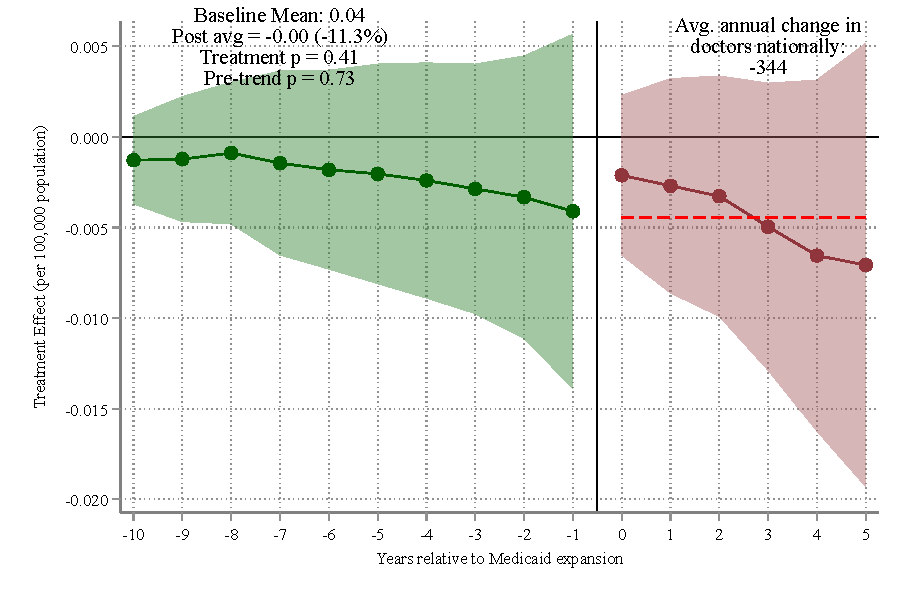
\includegraphics[width=0.75\linewidth]{figures/appx-quota-specialty-nonprimary.pdf}
        \caption{Non-Primary Care Positions}
        \label{afig6:non-prim-care}
    \end{subfigure}
    \hfill
    \begin{subfigure}{\linewidth}
        \centering
        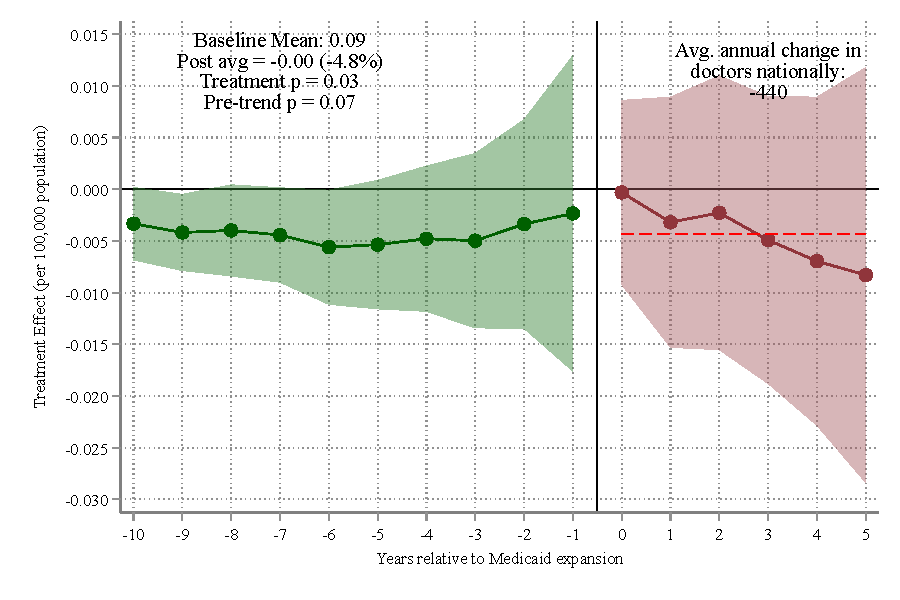
\includegraphics[width=0.75\linewidth]{figures/appx-quota-specialty-primary.pdf}
        \caption{Primary Care Positions}
        \label{afig6:prim-care}
    \end{subfigure}
\caption*{\footnotesize{\textit{Notes:} The figure plots event-study coefficients from the imputation estimator of Borusyak, Jaravel, and Spiess (2024), estimated separately for non-primary care (top panel) and primary care specialties (bottom panel). The outcome is quota positions per 100,000 state population, where quota measures positions offered by programs prior to the matching algorithm. For non-primary care, the average post-expansion treatment effect is $-0.00$ ($-9.7$ percent relative to the pre-expansion mean of $0.04$; p $= 0.12$), corresponding to an average annual reduction of approximately $193$ offered positions nationally. For primary care, the average treatment effect is $-0.01$ ($-9.3$ percent relative to the pre-expansion mean of $0.07$; p $< 0.01$), corresponding to an average annual reduction of approximately $554$ offered positions. Shaded bands are 95 percent confidence intervals. Regressions include hospital and year fixed effects. Standard errors are clustered at the state level.}}
\end{figure}


\begin{figure}[H]
    \caption{Robustness of Event Study Estimates Across Difference-in-Differences Estimators, Total Matched Residency Positions in Levels}
    \label{afig7}
    \centering
      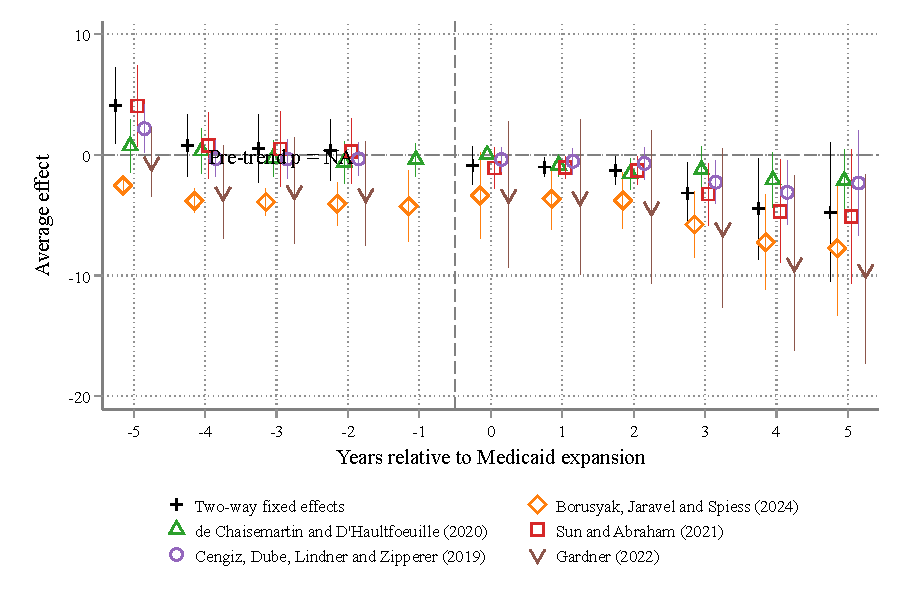
\includegraphics[width=\linewidth]{figures/appx-estimators-levels.pdf}
    \hfill
\caption*{\footnotesize{\textit{Notes:} The figure compares event-study estimates of the effect of Medicaid expansion on the absolute number of matched residency positions per hospital across six difference-in-differences estimators that are robust to treatment-effect heterogeneity under staggered adoption: two-way fixed effects; Borusyak, Jaravel, and Spiess (2024); de Chaisemartin and D'Haultfoeuille (2020); Sun and Abraham (2021); Cengiz, Dube, Lindner, and Zipperer (2019); and Gardner (2022). The heterogeneity-robust estimator of Callaway and Sant'Anna (2021) is excluded because it is not well identified in the sparsely populated never-treated cells of this sample. The pre-trend $p$-value reported in the panel is from the Borusyak, Jaravel, and Spiess (2024) estimator. The dashed vertical line marks the expansion year. Regressions include hospital and year fixed effects. Standard errors are clustered at the state level.}}
\end{figure}

\begin{figure}[H]
    \caption{Robustness of Event Study Estimates Across Difference-in-Differences Estimators, Residency Quota Positions per 100,000 Population}
    \label{afig8}
    \centering
      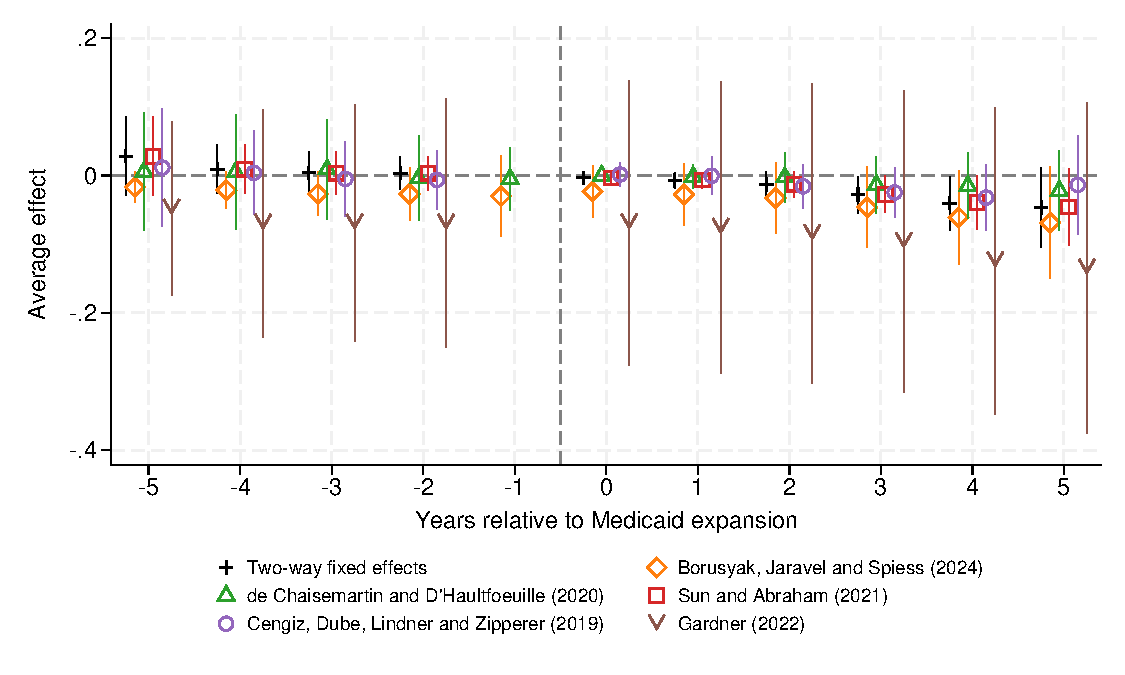
\includegraphics[width=\linewidth]{figures/appx-estimators-quota.pdf}
    \hfill
\caption*{\footnotesize{\textit{Notes:} The figure compares event-study estimates of the effect of Medicaid expansion on quota positions per 100,000 state population across six difference-in-differences estimators. Quota positions measure positions offered by residency programs prior to the matching algorithm. The estimators are: two-way fixed effects; Borusyak, Jaravel, and Spiess (2024); de Chaisemartin and D'Haultfoeuille (2020); Sun and Abraham (2021); Cengiz, Dube, Lindner, and Zipperer (2019); and Gardner (2022); the Callaway and Sant'Anna (2021) estimator is excluded as in the previous figure. The dashed vertical line marks the expansion year. Regressions include hospital and year fixed effects. Standard errors are clustered at the state level.}}
\end{figure}

\begin{figure}[H]
    \caption{Effect of Medicaid Expansion on Matched Residency Positions (Unweighted): Event Study Estimates}
    \label{afig10}
    \centering
      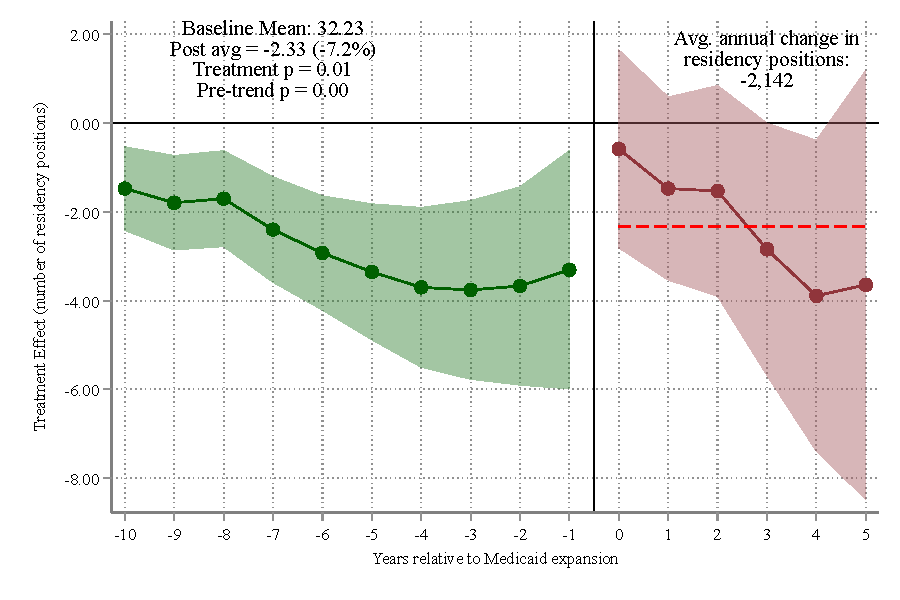
\includegraphics[width=\linewidth]{figures/appx-popcount-levels.pdf}
    \hfill
\caption*{\footnotesize{\textit{Notes:} The figure plots event-study coefficients from the imputation estimator of Borusyak, Jaravel, and Spiess (2024), where the outcome is the number of matched residency positions. This specification is estimated without population weights and includes 2010 state population as a control. The horizontal axis measures years relative to a state's Medicaid expansion; year 0 is the first year of expansion. Green circles (years $-5$ to $-1$) show pre-expansion coefficients. Dark red circles (years $0$ to $+5$) show post-expansion treatment effects. The dashed red line indicates the average post-expansion treatment effect ($-2.49$), which corresponds to approximately $-8.5$ percent relative to the pre-expansion mean of $29.42$ matched positions (p-value $= 0.00$). Translating to aggregate counts, expansion states experienced an average annual reduction of approximately $1{,}610$ matched residency positions relative to the counterfactual. Shaded bands are 95 percent confidence intervals. Regressions include hospital and year fixed effects. Standard errors are clustered at the state level.}}
\end{figure}

\begin{figure}[H]
    \caption{Effect of Medicaid Expansion on Matched Residency Positions per 100,000 Population (Unweighted): Event Study Estimates}
    \label{afig11}
    \centering
      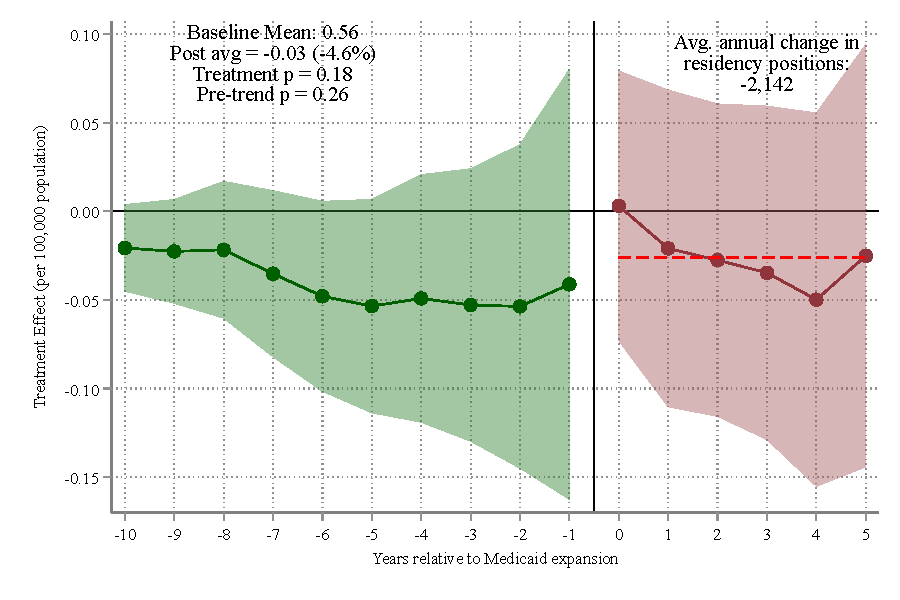
\includegraphics[width=\linewidth]{figures/appx-popcount-percapita.pdf}
    \hfill
\caption*{\footnotesize{\textit{Notes:} The figure plots event-study coefficients from the imputation estimator of Borusyak, Jaravel, and Spiess (2024), where the outcome is matched residency positions per 100,000 state population. This specification is estimated without population weights and includes 2010 state population as a control. The horizontal axis measures years relative to a state's Medicaid expansion; year 0 is the first year of expansion. Green circles (years $-5$ to $-1$) show pre-expansion coefficients. Dark red circles (years $0$ to $+5$) show post-expansion treatment effects. The dashed red line indicates the average post-expansion treatment effect ($-0.02$), which corresponds to approximately $-3.7$ percent relative to the pre-expansion mean of $0.51$ matched positions per 100,000 (p-value $= 0.34$). Translating to aggregate counts, expansion states experienced an average annual reduction of approximately $1{,}610$ matched residency positions relative to the counterfactual. Shaded bands are 95 percent confidence intervals. Regressions include hospital and year fixed effects. Standard errors are clustered at the state level.}}
\end{figure}

\begin{figure}[H]
    \caption{Effect of Medicaid Expansion on Residency Quota Positions per 100,000 Population (Unweighted): Event Study Estimates}
    \label{afig12}
    \centering
      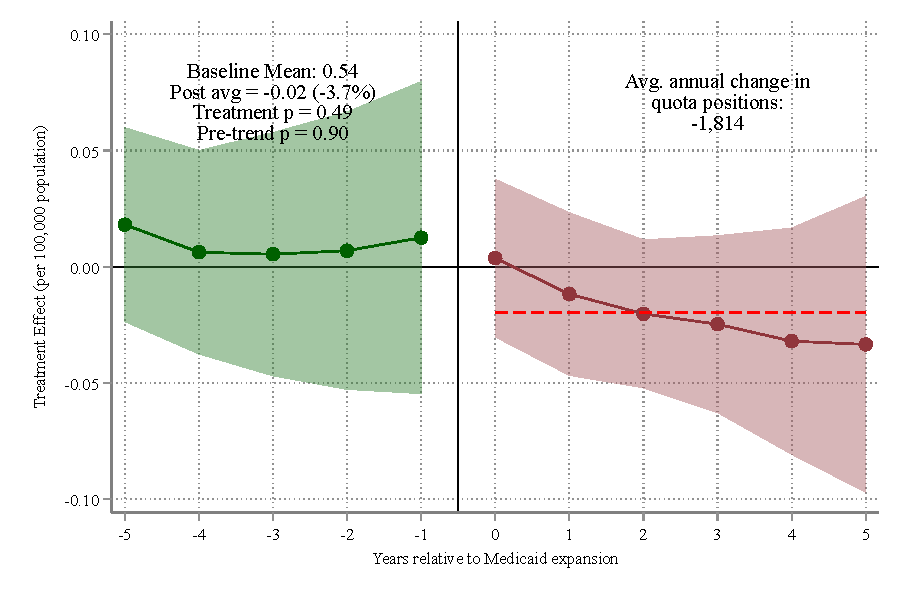
\includegraphics[width=\linewidth]{figures/appx-popcount-quota.pdf}
    \hfill
\caption*{\footnotesize{\textit{Notes:} The figure plots event-study coefficients from the imputation estimator of Borusyak, Jaravel, and Spiess (2024), where the outcome is residency quota (offered) positions per 100,000 state population. This specification is estimated without population weights and includes 2010 state population as a control. The horizontal axis measures years relative to a state's Medicaid expansion; year 0 is the first year of expansion. Green circles (years $-5$ to $-1$) show pre-expansion coefficients. Dark red circles (years $0$ to $+5$) show post-expansion treatment effects. The dashed red line indicates the average post-expansion treatment effect ($-0.02$), which corresponds to approximately $-3.7$ percent relative to the pre-expansion mean of $0.54$ quota positions per 100,000 (p-value $= 0.49$). Translating to aggregate counts, expansion states experienced an average annual reduction of approximately $1{,}814$ quota residency positions relative to the counterfactual. Shaded bands are 95 percent confidence intervals. Regressions include hospital and year fixed effects. Standard errors are clustered at the state level.}}
\end{figure}

\begin{figure}[H]
    \caption{Group-Specific Payment Evidence: Effect of Medicaid Expansion on Direct GME (DGME) Payments by State Medicaid GME Formula}
    \label{afig:fs_dgme}
    \centering
    \begin{subfigure}{\linewidth}
        \centering
        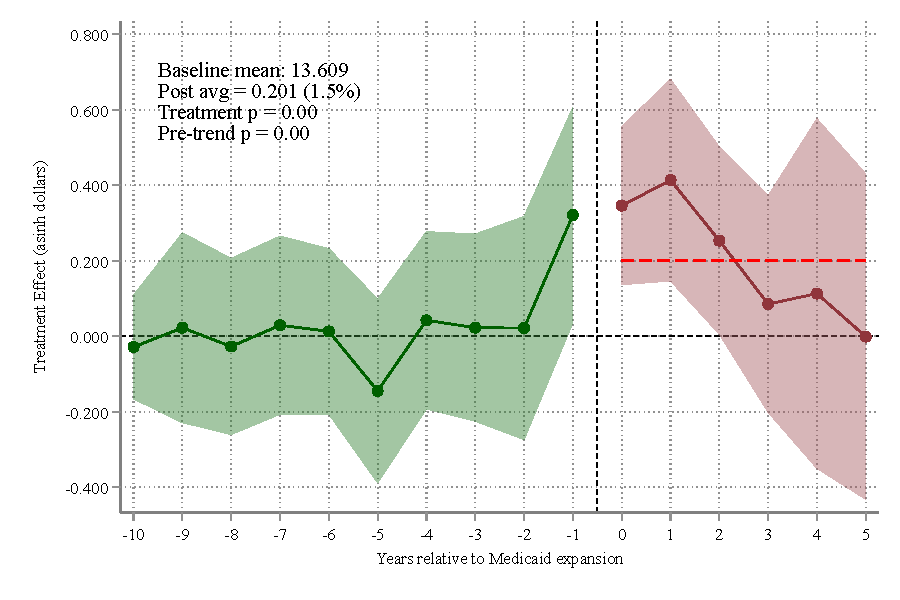
\includegraphics[width=0.75\linewidth]{figures/appx-firststage-dgme-volume.pdf}
        \caption{Volume-Responsive GME States}
        \label{afig:fs_dgme:vol}
    \end{subfigure}
    \hfill
    \begin{subfigure}{\linewidth}
        \centering
        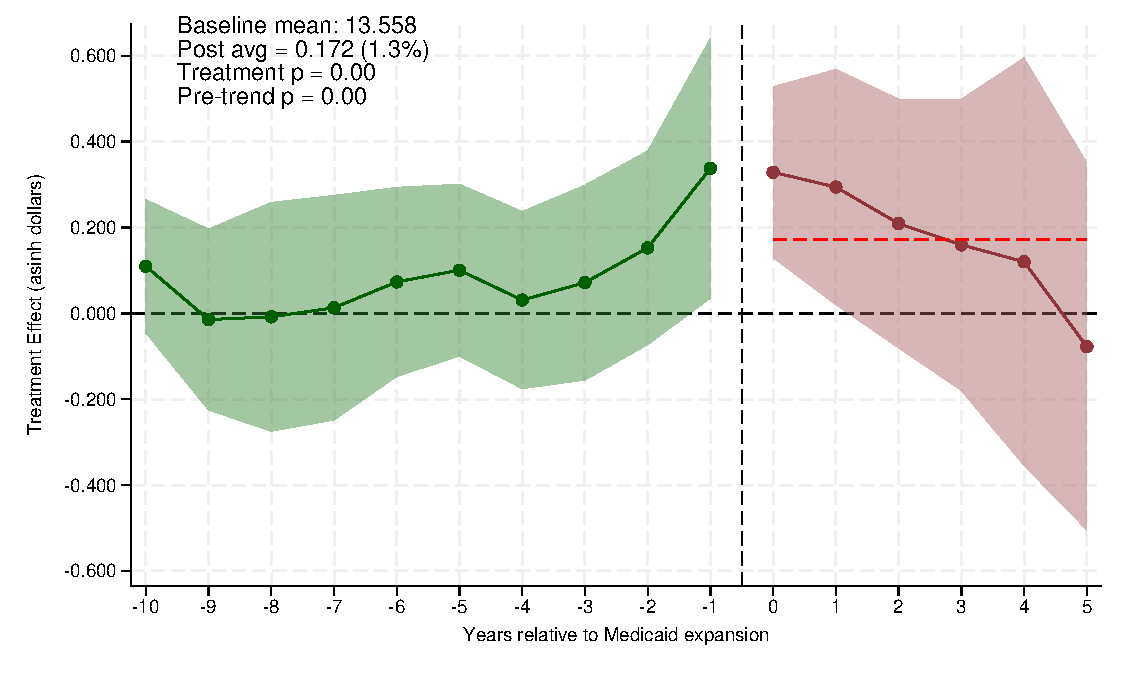
\includegraphics[width=0.75\linewidth]{figures/appx-firststage-dgme-nonresp.pdf}
        \caption{Non-Responsive GME States (Fixed/None)}
        \label{afig:fs_dgme:nonresp}
    \end{subfigure}
\caption*{\footnotesize{\textit{Notes:} The figure re-estimates the Direct GME (DGME) payment event study from \cref{afig13} separately for volume-responsive (top) and non-responsive (bottom) expansion states, each using never-expansion states as the comparison group. The outcome is Medicare cost-report payments, which we read as a proxy for training-related revenue rather than a direct measure of state Medicaid GME payments (see \cref{subsec:mechanisms}). The outcome is the inverse hyperbolic sine (asinh) of DGME payments per teaching hospital, so coefficients approximate proportional changes. In volume-responsive states the average post-expansion effect is $0.24$ (s.e.\ $0.14$; roughly a $24$ percent increase; joint $p < 0.01$), but this panel fails its pre-trend test (pre-trend $p = 0.0002$), so its level should be read with caution; in non-responsive states the effect is $0.10$ (s.e.\ $0.12$; roughly $10$ percent; joint $p < 0.01$; pre-trend $p = 0.30$), less than half as large, though the cross-group difference is imprecise ($0.14$, s.e.\ $0.10$, $p = 0.15$ from a pooled interacted model); see \cref{afig:fs_ftes,afig:fs_perfte} for the FTE/rate decomposition, where the cross-group contrast is sharper. Green circles (years $-5$ to $-1$) show pre-expansion coefficients; dark red circles (years $0$ to $+5$) show post-expansion effects; the dashed red line marks the average post-expansion effect. Shaded bands are 95 percent confidence intervals. Estimates come from CMS Medicare hospital cost reports at the hospital--fiscal-year level. Regressions include hospital and year fixed effects and are unweighted. Standard errors are clustered at the state level.}}
\end{figure}

\begin{figure}[H]
    \caption{Group-Specific Payment Evidence: Effect of Medicaid Expansion on Indirect Medical Education (IME) Payments by State Medicaid GME Formula}
    \label{afig:fs_ime}
    \centering
    \begin{subfigure}{\linewidth}
        \centering
        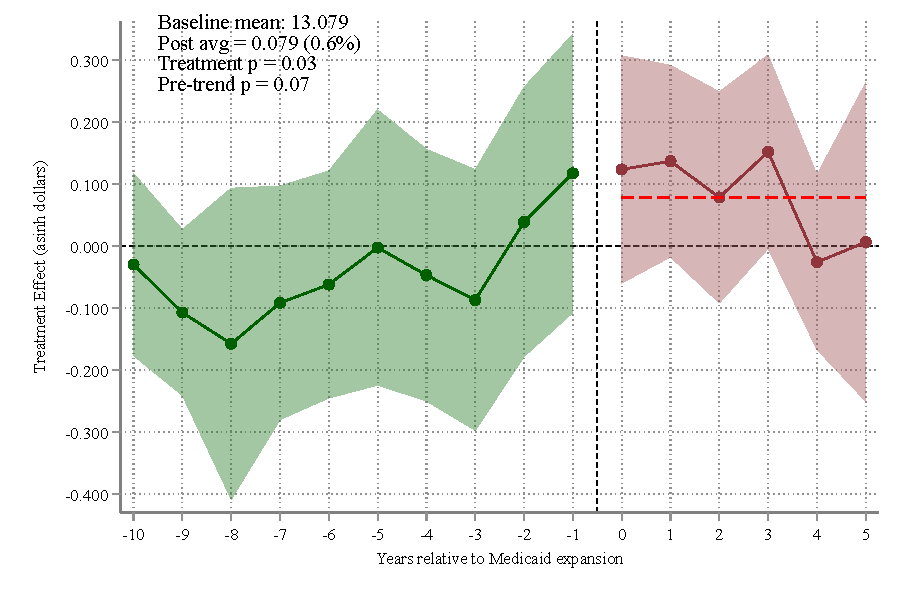
\includegraphics[width=0.75\linewidth]{figures/appx-firststage-ime-volume.pdf}
        \caption{Volume-Responsive GME States}
        \label{afig:fs_ime:vol}
    \end{subfigure}
    \hfill
    \begin{subfigure}{\linewidth}
        \centering
        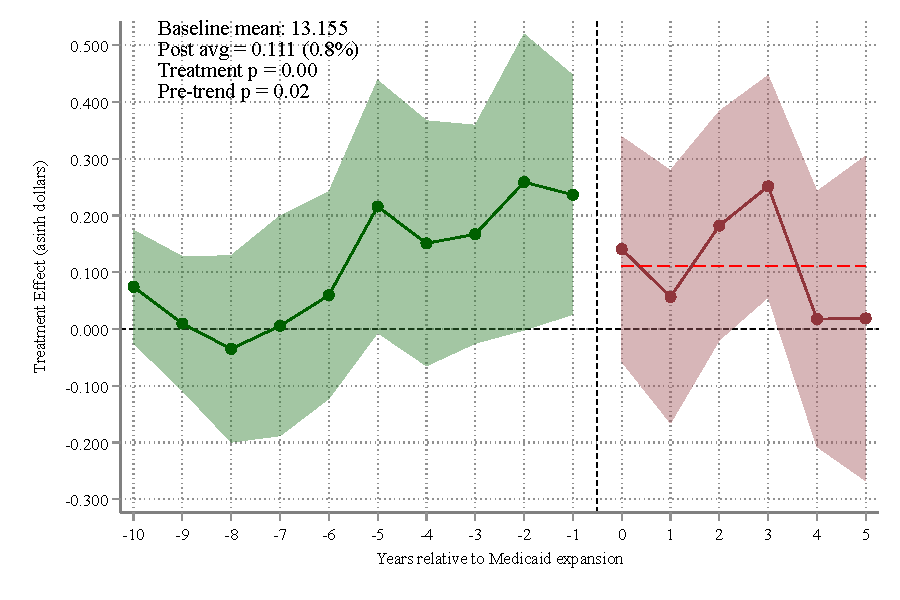
\includegraphics[width=0.75\linewidth]{figures/appx-firststage-ime-nonresp.pdf}
        \caption{Non-Responsive GME States (Fixed/None)}
        \label{afig:fs_ime:nonresp}
    \end{subfigure}
\caption*{\footnotesize{\textit{Notes:} The figure re-estimates the Indirect Medical Education (IME) payment event study from \cref{afig14} separately for volume-responsive (top) and non-responsive (bottom) expansion states, each using never-expansion states as the comparison group. The outcome is the inverse hyperbolic sine (asinh) of IME payments per teaching hospital, from Medicare cost reports (a proxy for training-related revenue; see \cref{subsec:mechanisms}). In volume-responsive states the average post-expansion effect is $0.17$ (s.e.\ $0.08$; roughly a $17$ percent increase; joint $p < 0.01$; pre-trend $p = 0.41$); in non-responsive states it is economically zero and statistically insignificant ($-0.003$, s.e.\ $0.07$; joint $p = 0.30$; pre-trend $p = 0.25$); the cross-group difference is significant ($0.15$, s.e.\ $0.05$, $p = 0.001$ from a pooled interacted model). The differential training-specific revenue gain from expansion is thus concentrated in the volume-responsive states, where residency positions do not contract. Green circles (years $-5$ to $-1$) show pre-expansion coefficients; dark red circles (years $0$ to $+5$) show post-expansion effects. Shaded bands are 95 percent confidence intervals. Regressions include hospital and year fixed effects and are unweighted. Standard errors are clustered at the state level.}}
\end{figure}

\begin{figure}[H]
    \caption{Decomposition of the DGME Payment Response: Resident FTEs by State Medicaid GME Formula}
    \label{afig:fs_ftes}
    \centering
    \begin{subfigure}{\linewidth}
        \centering
        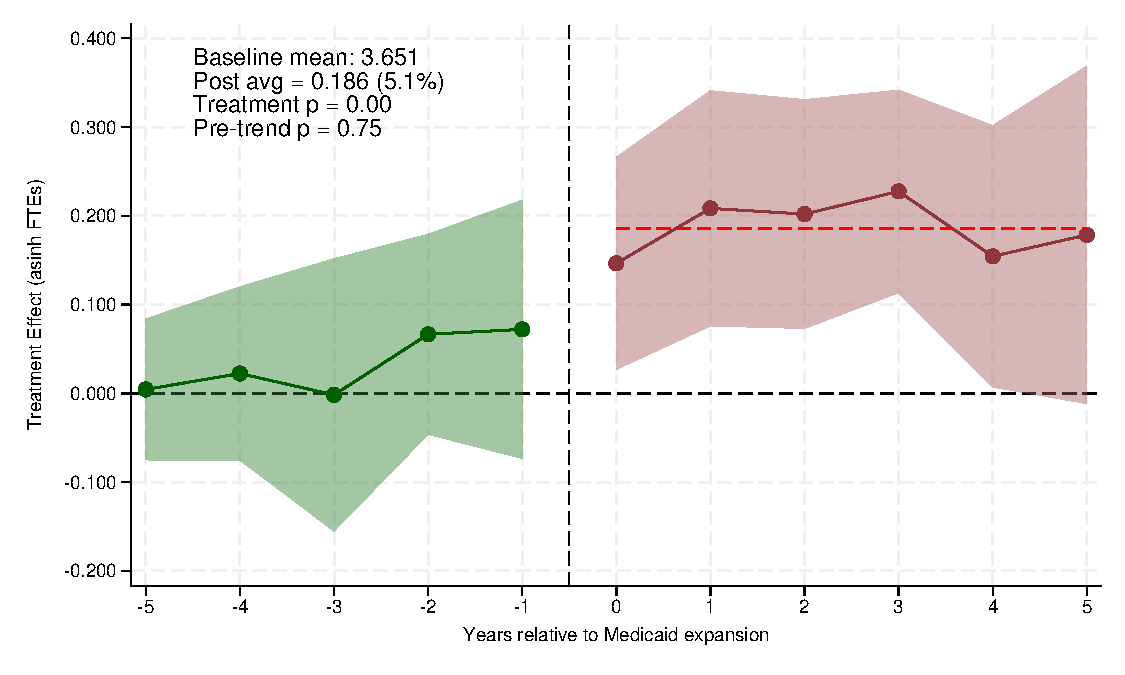
\includegraphics[width=0.75\linewidth]{figures/appx-firststage-dgmeftes-volume.pdf}
        \caption{Volume-Responsive GME States}
    \end{subfigure}
    \hfill
    \begin{subfigure}{\linewidth}
        \centering
        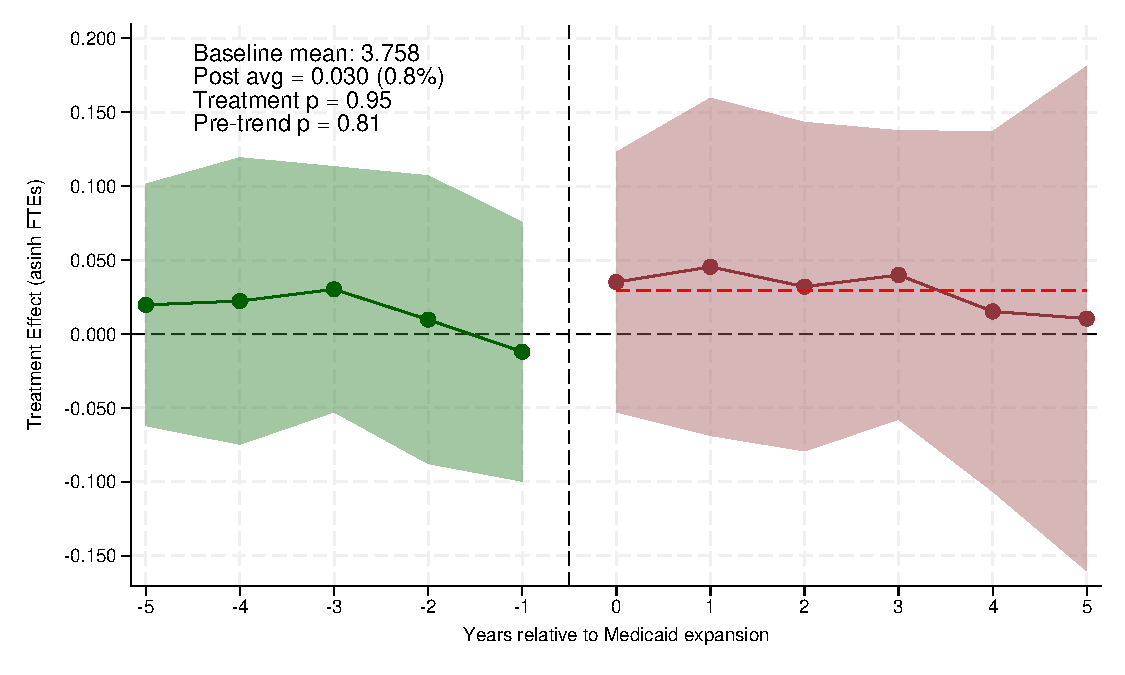
\includegraphics[width=0.75\linewidth]{figures/appx-firststage-dgmeftes-nonresp.pdf}
        \caption{Non-Responsive GME States (Fixed/None)}
    \end{subfigure}
\caption*{\footnotesize{\textit{Notes:} The figure decomposes the Direct GME payment response in \cref{afig:fs_dgme}: the outcome is the inverse hyperbolic sine of cost-report DGME resident FTEs per teaching hospital, so coefficients approximate proportional changes in the number of residents hospitals report for payment purposes. In volume-responsive states resident FTEs rise by roughly $19$ percent (average post effect $0.186$, s.e.\ $0.065$; joint $p < 0.001$) after flat pre-trends ($p = 0.75$); in non-responsive states FTEs do not move ($+3$ percent, s.e.\ $0.055$; joint $p = 0.95$; pre-trend $p = 0.81$). The cross-group difference is $0.14$ (s.e.\ $0.05$, $p = 0.005$ from a pooled interacted model). These estimates are on the full unweighted cost-report sample; on the linked NRMP--cost-report sample with the headline's weights and year convention the FTE response is negative in both arms (see \cref{subsec:inference} and the linked-sample reconciliation exhibits), so the unweighted rise here should not be read as evidence that training expanded. The DGME payment growth in volume-responsive states is therefore a quantity response, while the smaller payment rise in non-responsive states occurs without any growth in residents. Green circles (years $-5$ to $-1$) show pre-expansion coefficients; dark red circles (years $0$ to $+5$) show post-expansion effects. Shaded bands are 95 percent confidence intervals. Estimates come from CMS Medicare hospital cost reports at the hospital--fiscal-year level with never-expansion states as the comparison group. Regressions include hospital and year fixed effects and are unweighted. Standard errors are clustered at the state level.}}
\end{figure}

\begin{figure}[H]
    \caption{Decomposition of the DGME Payment Response: Payment per Resident FTE by State Medicaid GME Formula}
    \label{afig:fs_perfte}
    \centering
    \begin{subfigure}{\linewidth}
        \centering
        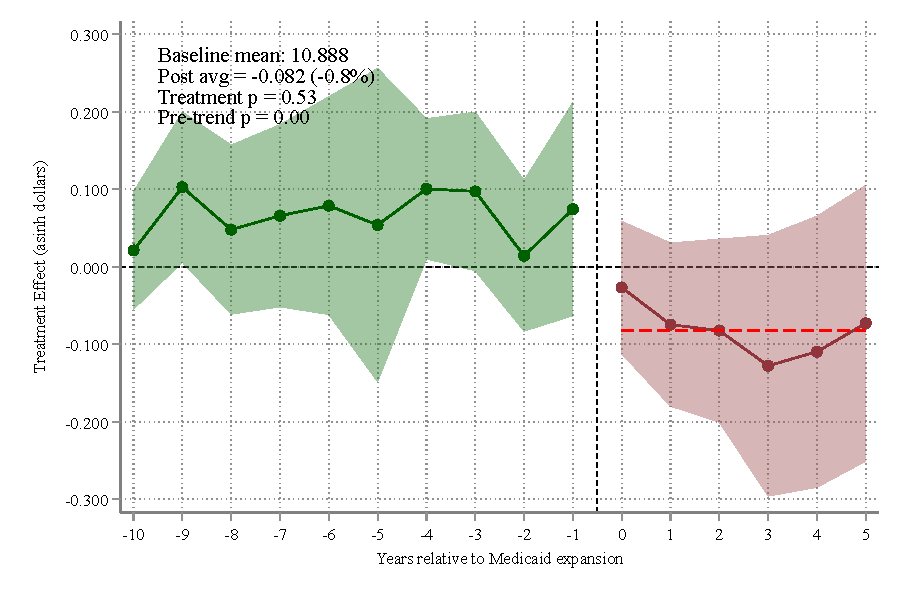
\includegraphics[width=0.75\linewidth]{figures/appx-firststage-dgmeperfte-volume.pdf}
        \caption{Volume-Responsive GME States}
    \end{subfigure}
    \hfill
    \begin{subfigure}{\linewidth}
        \centering
        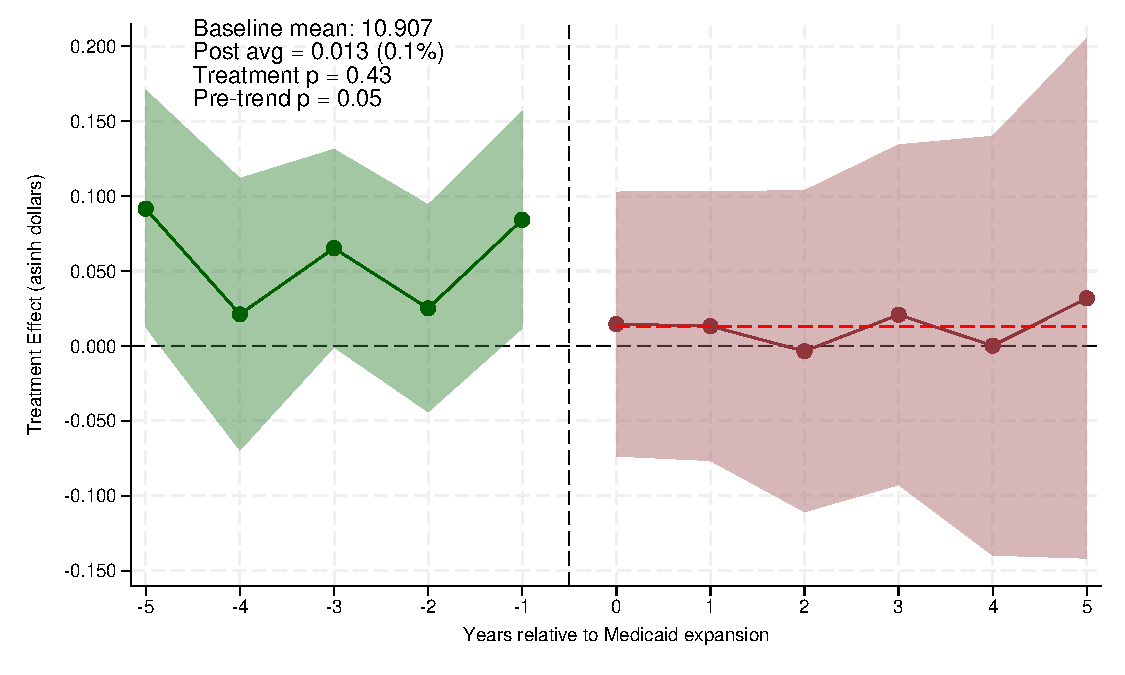
\includegraphics[width=0.75\linewidth]{figures/appx-firststage-dgmeperfte-nonresp.pdf}
        \caption{Non-Responsive GME States (Fixed/None)}
    \end{subfigure}
\caption*{\footnotesize{\textit{Notes:} The figure completes the decomposition in \cref{afig:fs_ftes}: the outcome is the inverse hyperbolic sine of DGME payment per resident FTE (hospitals with positive FTEs only). Per-FTE payments do not rise in either group: the average post effect is $-0.08$ in volume-responsive states (s.e.\ $0.06$; joint $p = 0.53$) and $+0.01$ in non-responsive states (s.e.\ $0.05$; joint $p = 0.43$; pre-trend $p = 0.053$); the cross-group difference is $-0.09$ (s.e.\ $0.04$, $p = 0.03$). The volume-responsive panel exhibits a differential pre-trend (pre-trend $p < 0.001$), so its level should be read with caution; the substantive conclusion---that the payment response is a quantity response, not a rate response---rests on the FTE panel. Green circles (years $-5$ to $-1$) show pre-expansion coefficients; dark red circles (years $0$ to $+5$) show post-expansion effects. Shaded bands are 95 percent confidence intervals. Estimates come from CMS Medicare hospital cost reports at the hospital--fiscal-year level with never-expansion states as the comparison group. Regressions include hospital and year fixed effects and are unweighted. Standard errors are clustered at the state level.}}
\end{figure}

\begin{figure}[H]
    \caption{Robustness to Not-Yet-Treated Controls: Effect of Medicaid Expansion on Matched Residency Positions per 100,000 Population}
    \label{afig:notyet}
    \centering
      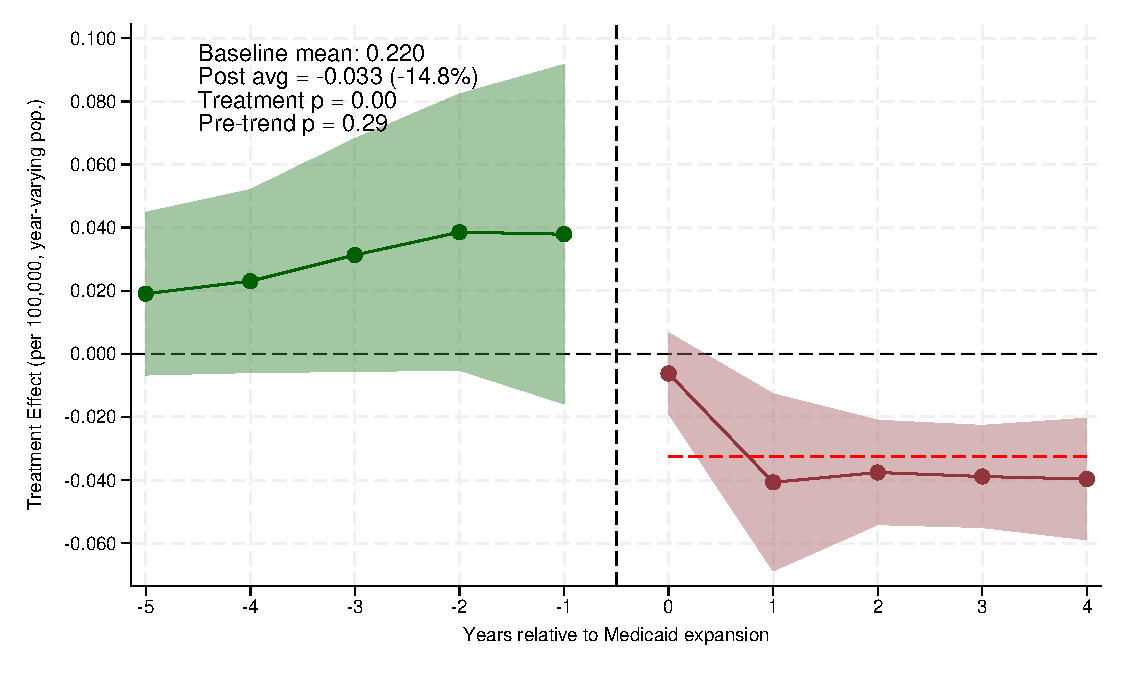
\includegraphics[width=\linewidth]{figures/appx-notyet.pdf}
    \hfill
\caption*{\footnotesize{\textit{Notes:} The figure re-estimates the main event study after dropping never-expansion states, so identification rests solely on variation in the timing of expansion among eventually-treated states (the not-yet-treated design). The outcome is matched positions per 100,000 contemporary (year-varying) population. Because the last-treated cohort has no valid comparison at horizon $+5$ under the not-yet-treated design, the event study is estimated over horizons $0$ to $+4$. The average post-expansion effect is $-0.033$ (a $14.8$ percent decline relative to the pre-expansion mean of $0.22$; joint clustered $p < 0.01$; randomization-inference $p = 0.38$, see \cref{subsec:inference})---larger and, under clustered inference, more precisely estimated than the full-sample effect---with flat pre-expansion coefficients (pre-trend $p = 0.29$). The contraction is therefore not an artifact of the never-expansion comparison group; if anything it is sharper when identification rests solely on the timing of expansion among adopters. Green circles (years $-5$ to $-1$) show pre-expansion coefficients; dark red circles (years $0$ to $+4$) show post-expansion effects; the dashed red line marks the average post-expansion effect. Shaded bands are 95 percent confidence intervals. Regressions include hospital and year fixed effects and weight by 2010 state population. Standard errors are clustered at the state level.}}
\end{figure}

\begin{figure}[H]
    \caption{Balanced-Cohort Event Study: 2014 Adopters Only}
    \label{afig:cohort2014}
    \centering
      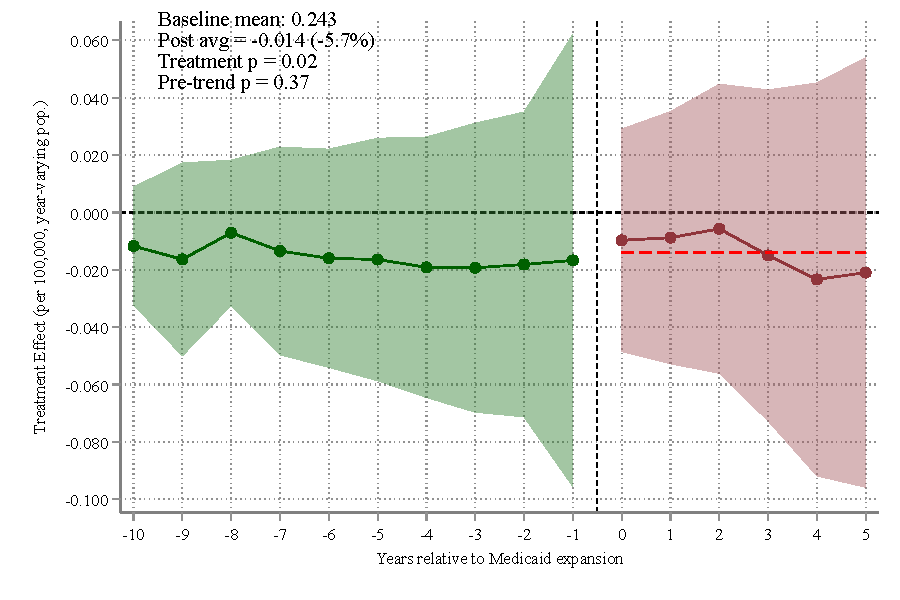
\includegraphics[width=\linewidth]{figures/appx-cohort2014.pdf}
    \hfill
\caption*{\footnotesize{\textit{Notes:} The figure re-estimates the main event study restricting treatment to the 2014 expansion cohort (the largest wave), with never-expansion states as the comparison group, so that every event-time coefficient is identified from the same fixed set of treated states. The outcome is matched positions per 100,000 contemporary (year-varying) population. The average post-expansion effect is $-0.015$ (a $7.5$ percent decline relative to the pre-expansion mean of $0.20$; joint $p = 0.16$ in this smaller single-cohort sample), and the event-time coefficients widen monotonically from $-0.004$ at horizon $0$ to $-0.024$ at horizon $+5$, following flat pre-expansion coefficients (pre-trend $p = 0.97$). Because cohort composition is held fixed, the widening path here reflects genuine dynamics rather than the changing composition of cohorts across horizons. Green circles (years $-5$ to $-1$) show pre-expansion coefficients; dark red circles (years $0$ to $+5$) show post-expansion effects; the dashed red line marks the average post-expansion effect. Shaded bands are 95 percent confidence intervals. Regressions include hospital and year fixed effects and weight by 2010 state population. Standard errors are clustered at the state level.}}
\end{figure}

\begin{figure}[H]
    \caption{Leave-One-State-Out Estimates of the Headline Effect}
    \label{afig:loo}
    \centering
      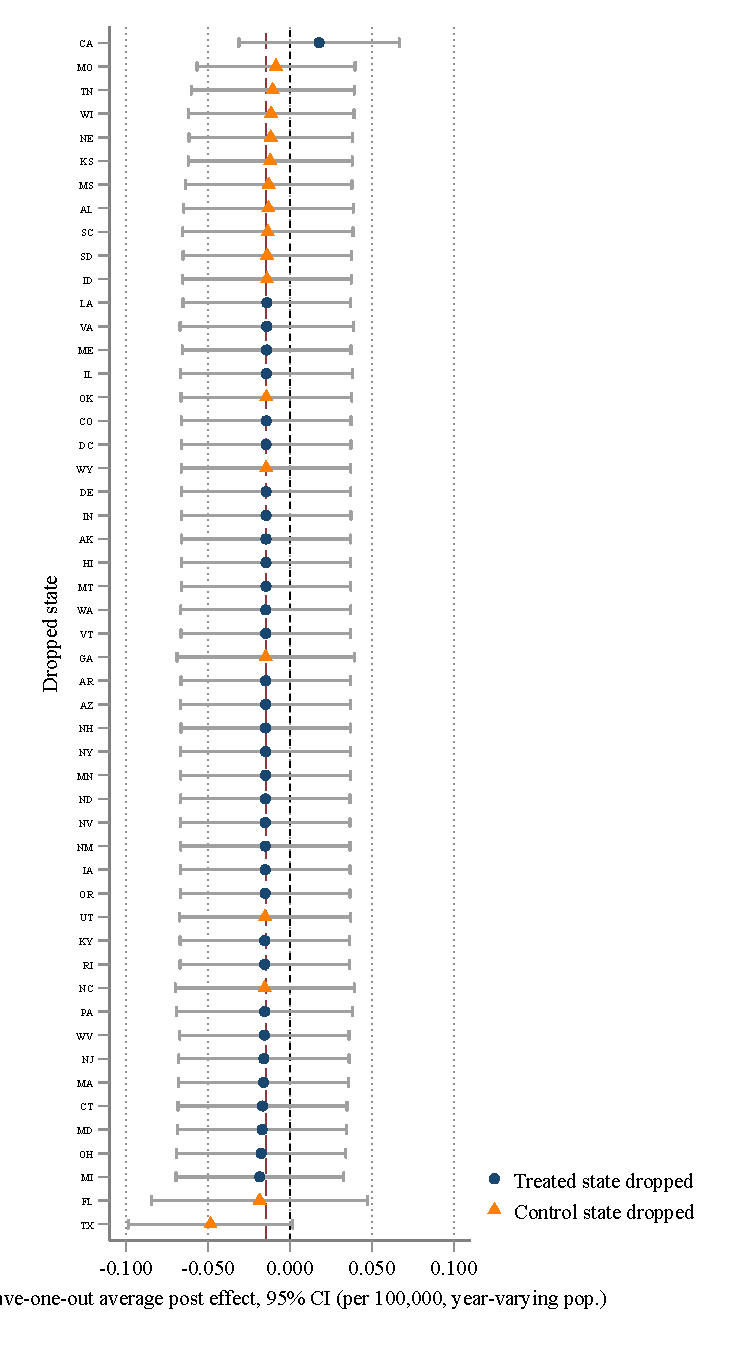
\includegraphics[width=0.8\linewidth]{figures/appx-loo.pdf}
    \hfill
\caption*{\footnotesize{\textit{Notes:} The figure plots the average post-expansion effect on matched positions per 100,000 contemporary (year-varying) population, re-estimated after dropping each treated state in turn (34 estimates, sorted). The dashed maroon line marks the full-sample estimate ($-0.016$); the thin black line marks zero. Every leave-one-out estimate remains negative (range $-0.018$ to $-0.001$), so the sign of the effect does not depend on any single state; dropping California alone, however, shrinks the estimate to $-0.001$, reflecting the concentration of identifying weight documented in \cref{subsec:inference}. Regressions include hospital and year fixed effects and weight by 2010 state population.}}
\end{figure}

\begin{figure}[H]
    \caption{HonestDiD Sensitivity to Violations of Parallel Trends}
    \label{afig:honest}
    \centering
    \begin{subfigure}{0.48\linewidth}
        \centering
        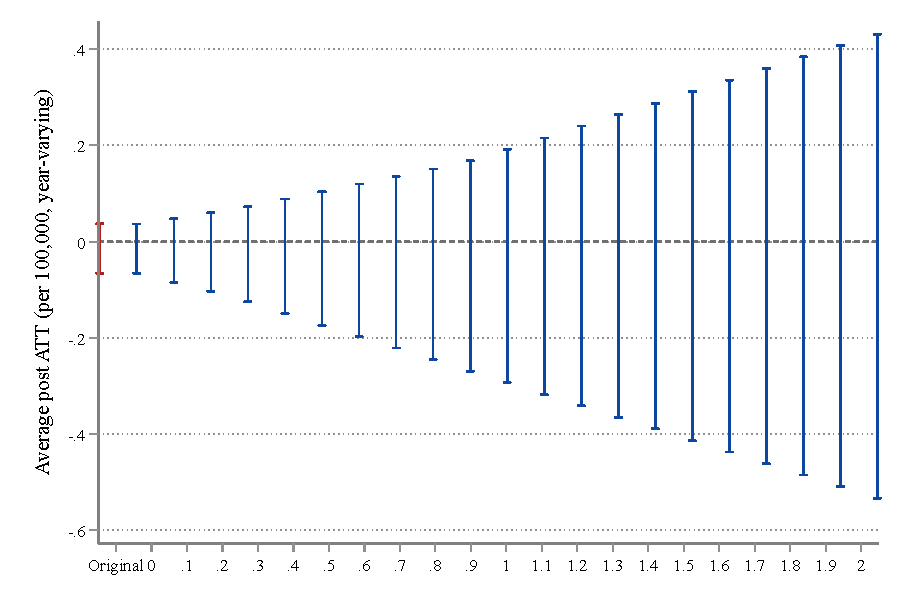
\includegraphics[width=\linewidth]{figures/appx-honestdid-headline.pdf}
        \caption{Headline (per 100,000, year-varying)}
        \label{afig:honest:head}
    \end{subfigure}
    \hfill
    \begin{subfigure}{0.48\linewidth}
        \centering
        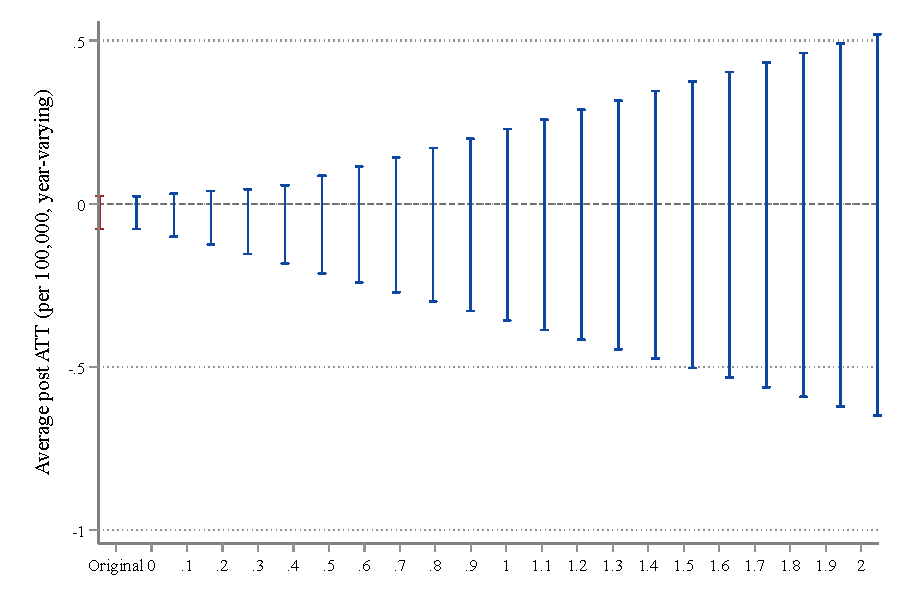
\includegraphics[width=\linewidth]{figures/appx-honestdid-nonresp.pdf}
        \caption{Non-Responsive States}
        \label{afig:honest:nonresp}
    \end{subfigure}
    \begin{subfigure}{0.48\linewidth}
        \centering
        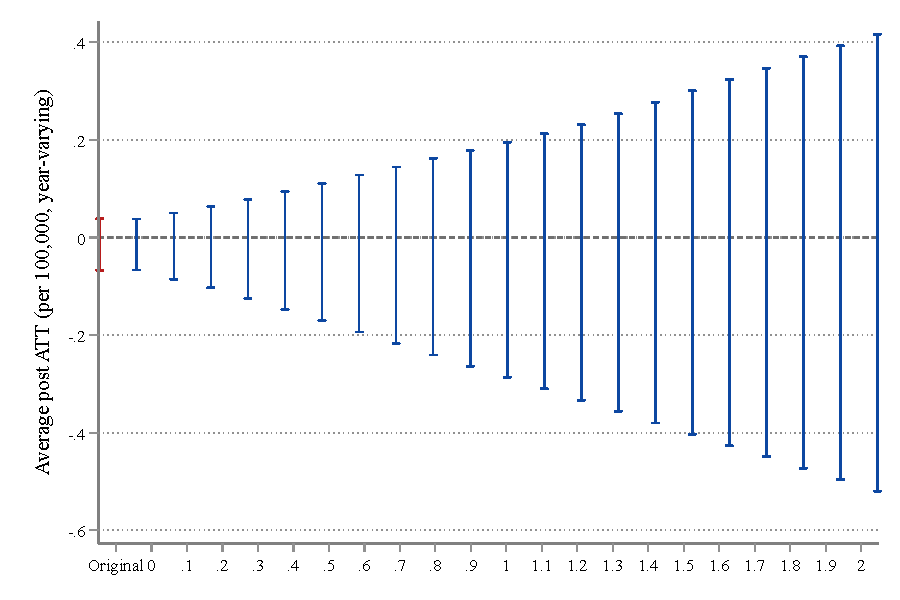
\includegraphics[width=\linewidth]{figures/appx-honestdid-urban.pdf}
        \caption{Urban Hospitals}
        \label{afig:honest:urban}
    \end{subfigure}
\caption*{\footnotesize{\textit{Notes:} The figure reports \textcite{rambachan2023more} sensitivity analysis for the average post-expansion effect on matched positions per 100,000 contemporary population, under the relative-magnitudes restriction $\Delta^{RM}(\bar{M})$, which bounds the post-period differential trend by $\bar{M}$ times the largest pre-period differential trend. Each panel plots the robust 95 percent confidence interval for the average post ATT as $\bar{M}$ increases. For the headline effect, the non-responsive mechanism panel, and the urban subsample, the robust confidence interval includes zero even at $\bar{M} = 0$ (exact parallel trends), confirming that the average magnitude is not distinguishable from zero at conventional levels; what the design supports is the sign and the growing dynamic path of the effect, together with the clustered joint tests and the not-yet-treated estimate. The leftmost interval in each panel is the original CI. Estimates use the Borusyak, Jaravel, and Spiess (2024) event-study coefficients with state-clustered standard errors.}}
\end{figure}

\newpage
\pagebreak
